\documentclass[a4paper]{article}
\usepackage[spanish]{babel}
\usepackage[utf8]{inputenc}
\usepackage{graphicx}
\usepackage{enumerate}
\usepackage{listings}
\usepackage{color}
\usepackage{indentfirst}
\usepackage{fancyhdr}
\usepackage{latexsym}
\usepackage{subfigure}
\usepackage[colorlinks=true, linkcolor=black]{hyperref}
%\usepackage{makeidx}
%\usepackage{float}
\usepackage{wrapfig}
\usepackage{calc}
\usepackage{amsmath, amsthm, amssymb}
\usepackage{amsfonts}
%\lstset{language=C}
\definecolor{gray}{gray}{0.5}
\definecolor{light-gray}{gray}{0.95}
\definecolor{orange}{rgb}{1,0.5,0}

\usepackage{fancyhdr}
\pagestyle{fancy}

%\renewcommand{\chaptermark}[1]{\markboth{#1}{}}
\renewcommand{\sectionmark}[1]{\markright{\thesection\ - #1}}

\fancyhf{}

\fancyhead[LO]{Sección \rightmark} % \thesection\ 
\fancyfoot[LO]{\small{Yanet Giuseppin, Laura Muiño, Javier San Miguel, Axel Straminsky}}
\fancyfoot[RO]{\thepage}
\renewcommand{\headrulewidth}{0.5pt}
\renewcommand{\footrulewidth}{0.5pt}
\setlength{\hoffset}{-0.8in}
\setlength{\textwidth}{16cm}
%\setlength{\hoffset}{-1.1cm}
%\setlength{\textwidth}{16cm}
\setlength{\headsep}{0.5cm}
\setlength{\textheight}{25cm}
\setlength{\voffset}{-0.7in}
\setlength{\headwidth}{\textwidth}
\setlength{\headheight}{13.1pt}

\renewcommand{\baselinestretch}{1.1}  % line spacing


% \setcounter{secnumdepth}{2}
\usepackage{underscore}
\usepackage{caratula}
\usepackage{url}
\usepackage{float}
\usepackage{algorithm}
\usepackage[noend]{algpseudocode}





\newcommand{\cod}[1]{{\tt #1}}
\newcommand{\negro}[1]{{\bf #1}}
\newcommand{\ital}[1]{{\em #1}}
\newcommand{\may}[1]{{\sc #1}}
\newcommand{\tab}{\hspace*{2em}}

%agrego para obtener nueracion por letras, despues verifico si funca
\renewcommand{\labelenumi}{[\alph{enumi}]}
\renewcommand{\labelenumii}{[\roman{enumii}]}

\hypersetup{
 pdfstartview= {FitH \hypercalcbp{\paperheight-\topmargin-1in-\headheight}},
 pdfauthor={Grupo},
 pdfsubject={Dise\~{n}o}
}

\lstdefinestyle{customc}{
  backgroundcolor=\color{light-gray},
  belowcaptionskip=1\baselineskip,
  breaklines=true,
  numbers=left,
  xleftmargin=\parindent,
  language=C,
  showstringspaces=false,
  basicstyle=\footnotesize\ttfamily,
  keywordstyle=\bfseries\color{blue},
  commentstyle=\itshape\color{gray},
  identifierstyle=\color{black},
  stringstyle=\color{orange},
}

\lstdefinestyle{customasm}{
  backgroundcolor=\color{light-gray},
  belowcaptionskip=1\baselineskip,
  numbers=left,
  xleftmargin=\parindent,
  language=[x86masm]Assembler,
  keywordstyle=\bfseries\color{blue},
  basicstyle=\footnotesize\ttfamily,
  commentstyle=\itshape\color{gray},
}

\lstset{escapechar=@}


\begin{document}

\thispagestyle{empty}
\materia{Métodos Numéricos}
\submateria{Segundo Cuatrimestre de 2015}
\titulo{Trabajo Práctico III}
%\subtitulo{Scheduling}
\integrante{Yanet Giuseppin}{184/11}{yanetagiu@yahoo.com}
\integrante{Laura Muiño}{399/11}{mmuino@dc.uba.ar}
\integrante{Javier San Miguel}{786/10}{javiersm00@gmail.com}
\integrante{Axel Straminsky}{769/11}{axelstraminsky@gmail.com}

\makeatletter

\maketitle
\newpage

\thispagestyle{empty}
\vfill

\thispagestyle{empty}
\vspace{3cm}
\tableofcontents
\newpage

\newenvironment{myindentpar}[1]
{\begin{list}{1}
         {\setlength{\leftmargin}{#1}}
         \item[]
}
{\end{list} }

%\normalsize
\newpage


\section{Introducción}

El objetivo de este trabajo es mostrar distintos métodos para generar videos en cámara lenta, a partir de otros videos.


Un video es una secuencia de imagenes, tambien llamados $frames$ o cuadros.  Las imagenes son matrices de pixeles (números que representan colores) y se muestran con una determinada velocidad de $frames$ por segundo (fps). Mientras más imagenes se muestren por segundo, mejor se ven los movimientos en el video, y mas fluidos.


Para darle un aspecto de $slow$ $motion$ a un video (cámara lenta), lo que se hace es agregar $frames$ entre los $frames$ originales del video. Como se conservan los fps del video, esto hace que el video resultante dure mas y los movimientos se vean más lentos. 

Si se agregaran $frames$ y se conservara la duración total del video, los fps incrementarían y el video se vería a la misma velocidad pero con movimientos mas fluidos y definidos.

 Queremos que los $frames$ que se agregan tengan alguna relación con los $frames$ originales entre los que se encuentran, aparentando ser $frames$ tomados tambien por la cámara de video.

Hay distintos métodos para generar los $frames$ que se van a agregar. Para este trabajo implementamos tres de ellos:

\begin{itemize}
\item Método del vecino más cercano: Los nuevos cuadros son copias del cuadro original más cercano.
\item Método de interpolación lineal, es el método de interpolación fragmentaria que utiliza polinomios lineales para aproximar los pixeles de los nuevos cuadros.
\item Método de interpolación cúbica, al igual que la interpolación lineal, es fragmentaria, sin embargo utiliza polinomios cúbicos para aproximar los cuadros a generar.
\end{itemize}

 Cada uno de los métodos tiene sus ventajas y desventajas particulares. Analizaremos los resultados obtenidos con videos de prueba para poder compararlos entre ellos y ver en qué casos uno es mejor que el otro, y en qué casos los $frames$ resultantes no son buenos.

 Para saber si los $frames$ generados se aproximan bien, se le quitan frames intermedios a los videos de entrada y con los métodos se generan esos mismos $frames$ que faltan. Luego comparamos los que generamos con los que quitamos del video original. Para compararlos usamos dos medidas: ECM (error cuadrático medio) y PSNR (del inglés Peak Signal-to-Noise Ratio).

 También vamos a analizar cuándo se producen $artifacts$ (errores visuales en las imágenes del video) debido a la aplicación de nuestros métodos. 

\newpage

\section{Desarrollo}

Cada método aproxima cada pixel de los $frames$ nuevos utilizando los pixeles de los $frames$ originales del video, y lo hace utilizando una función matemática. 
Por ejemplo, para generar el valor del pixel en la posición (i,j) de un nuevo $frame$, se utilizan los valores de los pixeles de los frames originales en la misma posicion (i,j). 

En el caso del método del vecino mas cercano hay solo dos valores posibles para un pixel. En los métodos lineal y cúbico ($splines$) se usan polinomios para hacer la aproximación.

\subsection{Método del vecino más cercano}
El algoritmo es bastante simple, cada $frame$ a agregar es la copia exacta del $frame$ original más cercano. Siendo $n$ la cantidad de $frames$ a agregar, cuando $n$ es par, se copia el frame $i$, $n/2$ veces y luego se copia el frame $i+1$ otras $n/2$. 

\begin{figure}[h!]
  \centering
    
\includegraphics[width=0.5\textwidth]{imagenes/genCopypar.png}
  \caption{Vecinos mas cercanos, agregando 2 frames}
\end{figure}

Cuando $n$ es impar, se copia el primer frame $n-1/2$ veces, y luego el resto de los frames se copia $n$ veces. Para el frame que está a igual distancia de los dos frames originales, utilizamos el frame posterior. No utilizamos ningún criterio en particular para esta decisión.

\begin{figure}[h!]
  \centering
    
\includegraphics[width=0.5\textwidth]{imagenes/genCopyImpar.png}
  \caption{Vecinos mas cercanos, agregando 3 frames}
\end{figure}

En las figuras anteriores, los cuadros con línea punteada son los frames interpolados, mientras que los frames con línea sin puntear son los frames originales.

\subsection{Método de interpolación lineal}
Se quiere aproximar con un polinomio de grado 1 (función lineal) los pixeles de los $frames$ que se agregan. Para estimar el valor del pixel $(i,j)$ en los nuevos frames, se utilizan los pixeles en la
misma posición $(i,j)$ de los $frames$ orginales anterior y posterior para construir el polinomio interpolador. \\

Si quisieramos agregar 2 frames nuevos, tomamos los valores del pixel en una posición determinada de los frames originales, que en el siguiente gráfico corresponde a los colores rojo y violeta, y a partir de ellos construimos una función lineal para averiguar los valores de los pixeles de los nuevos $frames$ (los de color azul y verde).


\begin{figure}[h!]
  \centering
    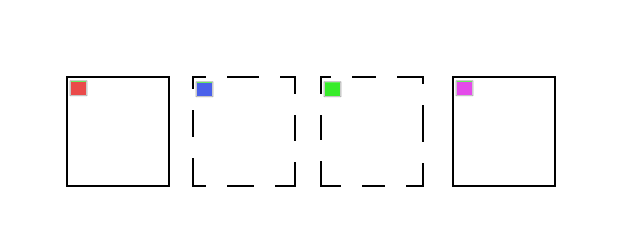
\includegraphics[width=0.5\textwidth]{imagenes/linealFrames.png}
  \caption{Gráfico de los pixeles de los frames originales e interpolados}
\end{figure}

Con los valores de esas posiciones construimos una función lineal para determinar los valores intermedios que deberán tomar pixeles de los $frames$ interpolados.

\begin{figure}[h!]
  \centering
    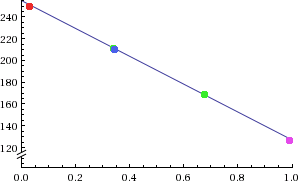
\includegraphics[width=0.5\textwidth]{imagenes/lineal2.png}
  \caption{Funcion lineal de acuerdo a los valores entre dos pixeles}
\end{figure}


El método equivale a encontrar los n-1 polinomios de primer grado $S_{j}$ que pasan por los puntos distintos $(x_{j},f(x_{j}))$ y $(x_{j+1},f(x_{j+1}))$ $\forall j \in (0,n-2)$.\\
En nuestro caso definimos los puntos $x_{0}, ... , x_{n-1}$ como el tiempo en que cada frame es reproducido. Por ejemplo, si tenemos un video a 24 fps, significa que en 1 segundo se muestran 24 frames. De este modo, sabemos que entre frame y frame hay una distancia temporal de 1/24 segundos. Estos son los valores que tomamos como los $x_{j}$ de nuestra función lineal. \\
Luego, ese intervalo se divide en intervalos equidistantes de acuerdo a la cantidad de frames que vayamos a agregar. Los valores $f(x_{j})$ equivalen al valor de un pixel del j-ésimo frame. 
%Es decir, se generan para cada pixel (i,j) de los n frames, n-1 polinomios.\\

%%%%%%%% imagen de toystory que explica lineal



\subsection{Interpolación cúbica o splines}
%SUPONEMOS QUE LA CANTIDAD DE FRAMES TOTALES (ORIGINALES) ES N+1, PARA QUE LOS ÍNDICES QUEDEN BONITOS.

Al igual que en el método de interpolación lineal, para las posiciones (i,j) de todos los frames del video, generamos los puntos intermedios a estos con splines, y asi generar las matrices de relleno posición a posición. Los $n+1$ puntos de interpolación $x_{0} .. x_{n}$ siguen representando el tiempo en el que cada frame es reproducido, dado por el framerate del video original.\\

Para construir los $n$ splines, se deben averiguar los valores de $4n$ constantes $a$, $b$, $c$ y $d$, correspondientes a los coeficientes de cada uno de los polinomios, con lo que se tiene bastante flexibilidad para asegurar que los splines construidos no solo son continuos y diferenciables en su intervalo, sino que tienen derivada segunda continua.\\
Primero recordaremos la definición de la interpolación cúbica por splines, para poder obtener propiedades a partir de ella: \\
Dada una función f: [a, b] y una sucesión de puntos $a= x_{0} < x_{1} < … < x_{n} = b$, una función interpolante cúbica S para f es una función que satisface las siguientes condiciones: \\

\begin{enumerate}
\item  S(x) es un polinomio de tercer grado, lo notamos como $S_{j}$ para el intervalo $[x_{j},x_{j+1}]$ $\forall j \in (0, n-1)$.
\item $S_{j}(x_{j})$ = $f(x_{j})$  y $S_{j}(x_{j+1})$ = $f(x_{j+1})$ $\forall j \int (0, n-1)$.
\item $S_{j+1}(x_{j+1})$ = $S_{j}(x_{j+1})$ $\forall j \in (0, n-2)$ (implicado por b)).
\item $S'_{j+1}(x_{j+1})$ = $S'_{j}(x_{j+1})$ $\forall j \in (0, n-2)$.
\item $S''_{j+1}(x_{j+1})$ = $S''_{j}(x_{j+1})$ $\forall j \in (0, n-2)$.
\item Alguna de las siguientes condiciones debe satisfacerse:
  \begin{enumerate}
  \item $S''(x_{0})$ = $S''(x_{n})$ = 0 (limite natural o libre).
  \item $S'(x_{0})$ = $f'(x_{0})$ y $S'(x_{n})$ = $f'(x_{n})$.
  \end{enumerate}
\end{enumerate}

En general la segunda condición del punto f) provee una aproximación más precisa porque incluye más información, sin embargo requeire los valores de la derivada de $f$ en los puntos de aproximación o una aproximación precisa de esos valores. Dado que no contamos con esta información, nos enfocamos en realizar un spline natural.\\


Construimos el spline aplicando las condiciones de la definición a los polinomios cúbicos\\ $S_{j}(x) = a_{j} + b_{j} (x - x_{j}) + c_{j} (x - x_{j})^{2} + d_{j} (x - x_{j})^{3}$ $\forall j \in (0, n-1)$.\\

Como $S_{j}$ = $a_{j}$ = $f(x_{j})$, la condición c) puede ser aplicada para obtener $ a_{j+1} = S_{j+1}(x_{j+1}) = S_{j}(x_{j+1}) = a_{j} + b_{j} (x_{j+1} - x_{j}) + c_{j} (x_{j+1} - x_{j})^{2} + d_{j} (x_{j+1} - x_{j})^{3}$ $\forall j \in (0, n-2)$.\\

Los términos $ x_{j+1} - x_{j} $ los renombraremos con la variable $h_{j}$ $\forall j \in (0, n-2)$ para mayor claridad. Si además llamamos $a_{n} = f(x_{n})$, entonces la ecuación

\begin{equation} \label{eq:ecuacion3.15}
a_{j+1} = a_{j} + b_{j} h_{j} + c_{j} h_{j}^{2} + d_{j} h_{j}^{3} 
\end{equation}

vale $\forall j \in (0, n-1)$. De manera similar, definiendo $b_{n} = S'(x_{n})$ se obtiene $S'_{j}(x) = b_{j} + 2c_{j} (x - x_{j}) + 3d_{j} (x - x_{j})^{2}$.
Si evaluamos en $x_{j}$ obtenemos  $S'_{j}(x_{j}) = b_{j}$, $\forall j \in (0, n-1)$. Si aplicamos la condición d) obtenemos

\begin{equation} \label{eq:ecuacion3.16}
b_{j+1} = b_{j} + 2c_{j} h_{j} + 3d_{j} h_{j}^{2}
\end{equation}

$\forall j \in (0, n-1)$. Otra relación entre los coeficientes de $S_{j}$ se obtiene definiendo $c_{n} = S''(x_{n})/2$ y luego aplicando la condición e). Tenemos que $\forall j \in (0, n-1)$ 

\begin{equation} \label{eq:ecuacion3.17}
c_{j+1} = c_{j} + 3d_{j} h_{j}.
\end{equation}

Despejando $d_{j}$ de la ecuación \ref{eq:ecuacion3.17} y reemplazando en las ecuaciones \ref{eq:ecuacion3.15} y \ref{eq:ecuacion3.16}, obtenemos que $\forall j \in (0, n-1)$ valen:\\

\begin{equation} \label{eq:ecuacion3.18}
a_{j+1} = a_{j} + b_{j} h_{j} + \frac{h_{j}^{2}}{3} (2c_{j} + c_{j+1})
\end{equation}
\begin{center} y \end{center}
\begin{equation} \label{eq:ecuacion3.19}
b_{j+1} = b_{j} + h_{j} (c_{j} + c_{j+1})
\end{equation}


Luego despejamos $b_{j}$ de la ecuación \ref{eq:ecuacion3.18} y reducimos el índice en uno, obteniendo 

\begin{equation} \label{eq:ecuacion3.20}
b_{j-1} = \frac{1}{h_{j-1}} (a_{j} - a_{j-1}) - \frac{h_{j-1}}{3} (2c_{j-1} + c_{j})                                
\end{equation}

Sustituimos $b_{j}$ y $b_{j-1}$ por sus valores correspondientes respecto a la ecuación \ref{eq:ecuacion3.19}. A continuación realizamos el despeje, para dar credibilidad a la cuestión:

$$b_{j} = b_{j-1} + h_{j-1} (c_{j-1} + c_{j})$$

$$\frac{1}{h_{j}} (a_{j+1} - a_{j}) - \frac{h_{j}}{3} (2c_{j} + c_{j+1}) = \frac{1}{h_{j-1}} (a_{j} - a_{j-1}) - \frac{h_{j-1}}{3} (2c_{j-1} + c_{j}) + h_{j-1} (c_{j-1} + c_{j})$$

$$ \frac{1}{h_{j}} (a_{j+1} - a_{j}) - \frac{1}{h_{j-1}} (a_{j} - a_{j-1}) = \frac{h_{j}}{3} (2c_{j} + c_{j+1}) - \frac{h_{j-1}}{3} (2c_{j-1} + c_{j}) + h_{j-1} (c_{j-1} + c_{j})$$

$$ \frac{3}{h_{j}} (a_{j+1} - a_{j}) - \frac{3}{h_{j-1}} (a_{j} - a_{j-1}) = h_{j} (2c_{j} + c_{j+1}) - h_{j-1} (2c_{j-1} + c_{j}) + 3h_{j-1} (c_{j-1} + c_{j}) $$

$$ \frac{3}{h_{j}} (a_{j+1} - a_{j}) - \frac{3}{h_{j-1}} (a_{j} - a_{j-1}) = 2h_{j}c_{j} + h_{j}c_{j+1} - 2h_{j-1}c_{j-1} - h_{j-1}c_{j} + 3h_{j-1}c_{j-1} + 3h_{j-1}c_{j} $$

$$ \frac{3}{h_{j}} (a_{j+1} - a_{j}) - \frac{3}{h_{j-1}} (a_{j} - a_{j-1}) = 2h_{j}c_{j} + h_{j}c_{j+1} + h_{j-1}c_{j-1} + 2h_{j-1}c_{j} $$

\begin{equation}\label{eq:ecuacion3.21}
 \frac{3}{h_{j}} (a_{j+1} - a_{j}) - \frac{3}{h_{j-1}} (a_{j} - a_{j-1}) = 2c_{j}(h_{j-1} + h_{j}) + h_{j-1}c_{j-1} + h_{j}c_{j+1} 
\end{equation}

$\forall j \in (1, n-1)$. \\

Las incógnitas de este sistema son los $\{c_{j}\}_{j=0}^{n}$. Los valores $\{ h_{j}\}_{j=0}^{n-1}$ y $\{ a_{j}\}_{j=0}^{n}$ están dados respectivamente por el espacio entre los puntos $\{x_{j}\}_{j=0}^{n}$ y los valores de f valuada en ellos. Una vez que los valores de $\{c_{j}\}_{j=0}^{n}$ son determinados, solo resta despejar $\{b_{j}\}_{j=0}^{n-1}$ de la ecuación \ref{eq:ecuacion3.20} y los $\{d_{j}\}_{j=0}^{n-1}$ de la ecuación \ref{eq:ecuacion3.17}. Con lo cual construimos los polinomios cúbicos $\{S_{j}(x)\}_{j=0}^{n-1}$. \\

El sistema planteado para buscar los valores $\{c_{j}\}_{j=0}^{n}$ los encuentra y además son únicos. La prueba de esto está formalizada en [BUR9].
\newpage

\section{Implementacion}

A la hora de implementar los métodos propuestos, decidimos incluir distintas variantes de los mismos. En primer lugar, implementamos los 3 métodos como mencionamos en la sección Desarrollo. Los parametros de nuestro programa son los siguientes: \\

\begin{itemize}
  \item $originalVideo.txt $: Archivo del video original en formato de texto.
  \item $generatedVideo.txt$: Archivo donde se guarda el video interpolado en formato de texto.
  \item $method$: Método de interpolación. Puede ser 0 (Vecinos más cercanos), 1 (Lineal) o 2 (Splines)
  \item $framesToAdd$: La cantidad de frames que se desea agregar entre 2 frames. Siempre se utiliza la misma cantidad de frames agregados entre dos frames. No se implementó una variante donde se agreguen más frames en un segmento del video que en otro.
  \item $checkVSoriginal$: Puede ser $true$ o $false$. En caso de ser $true$, toma el video original y remueve $framesToAdd$ frames, dejando un frame de por medio. Por ejemplo, si tengo un video de 11 frames y $framesToAdd$ es 2, el video a procesar constaría de los frames 0, 3, 6 y 9 (el último frame es removido, y se obtendrá un video más corto que el original de no ser justo un múltiplo). Se interpolarían esos frames, y además de devolder el video interpolado, devuelve el ECM y PSNR entre los frames generados y los frames originales que fueron removidos.\\
  Si es $false$, no se remueven frames del video original.
  \item $intervalMethod$: Puede ser $block$ o $ecm$. Si es $block$, divide al video original en segmentos del tamaño del parametro que sigue. Si es $ecm$, divide al video en segmentos de acuerdo al parametro que sigue.
  \item $blockSizeOrThreshold$: Si $intervalMethod$ es $block$, el parametro debe ser un entero que indica el tamaño de bloque en que se divide el video. Cada segmento tendrá tantos frames como indique este parámetro (excpeto el último segmento de no ser un múltiplo). El tamaño debe ser mayor a 1, dado que si se dividiera en bloques de 1 frame, no hay vídeo a interpolar. Si el tamaño es la cantidad de frames del video original o mayor, no se divide el video original en segmentos y se lo toma como un solo video. \\
  Si $intervalMethod$ es $ecm$, el parametro debe ser un numero real mayor o igual a cero. Este número indica el umbral a partir del cual se debe segmentar un video. Se recorre el video original, comparando el frame $i$ con el frame $i+1$. Si el ECM es mayor al parámetro, allí se debe segmentar el vídeo. La idea original era no procesar los frames donde hubiera un cambio brusco de cámara. Sin embargo no ahondamos en esta alternativa y en la implementación interpola entre esos frames también.
\end{itemize}

Cuando sacamos frames del video original, hacemos de cuenta que el video original en realidad tiene menos frames de los que realmente tiene. En la siguiente imagen, indicamos con una X los frames que removemos, los cuales serán los que generaremos con el método propuesto.

\begin{figure}[h!]
  \centering
    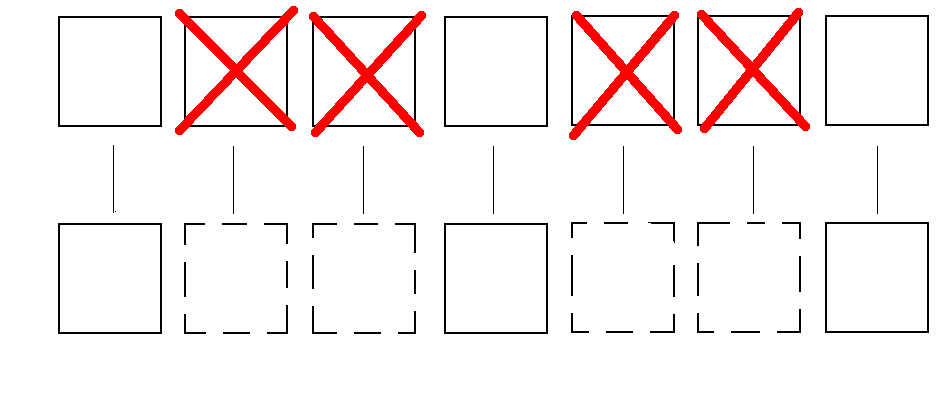
\includegraphics[scale= 0.3]{imagenes/sacandoFrames.png}
  \caption{Como se sacan frames del video original para comparar con los originales}
\end{figure}

Cuando segmentamos el video en bloques, el último frame de un bloque es el primer frame del bloque siguiente (excepto el último). Esto se debe a que, de no ser así, habria frames para los cuales no se interpolaría. Cuando se divide el método por bloques de igual tamaño, esto no parecería tener mucho sentido a menos que el video original justo tenga cambios de cámara en cada tamaño de bloque.

\begin{figure}[h!]
  \centering
    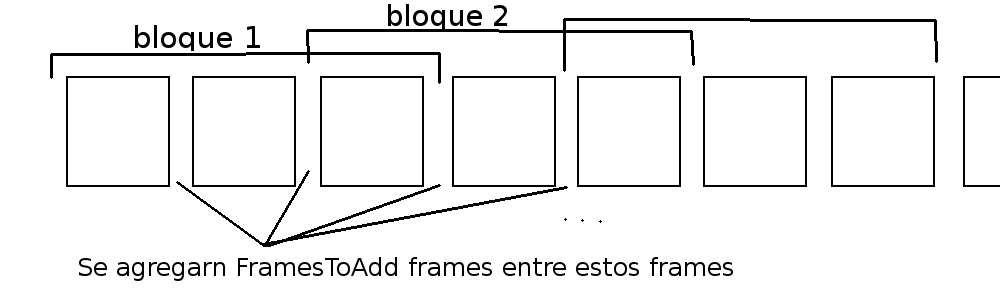
\includegraphics[scale= 0.3]{imagenes/framesToAddBloques.png}
  \caption{Como se segmenta el video en bloques}
\end{figure}


% \begin{algorithm}
% \caption{Método de la Potencia}\label{metpot}
% \begin{algorithmic}[1]

%   \Function{MetodoPotencia}{Matriz A, vector x, double c, tolerance, maxIter}%\Comment{con $A \in R^{(nxm)*(nxm)}$, $b \in R^{nxm}$}

%     \State $x = x/\lVert \mathbf{p} \rVert _{1}$
%     \While{ no se alcance la iteracion máxima}
%       \State resuelvo sistema y = A.(1-c)*x + ms
%       \State obtengo norma de y
%       \State  defino error como la norma uno de la resta entre x e y
%       \If {difieren en menos del error tolerado}
%         \State devuelvo vector y con su norma como autovalor
%       \Else
%         \State x = y
%       \EndIf
%     \EndWhile
%     \Return false
%   \EndFunction

% \end{algorithmic}
% \end{algorithm}


\newpage

\section{Experimentación}
Los primeros dos experimentos que veremos, se centran en el tiempo de ejecución de los procesos. Dichos experimentos tienen como finalidad estudiar como influye la cantidad de frames del video y la cantidad de frames a generar en el tiempo de ejecución, y si un video con mucho movimiento implica mayor tiempo de procesamiento que uno estático.\\

\subsection{Experimentación Temporal}

Como video de prueba, utilizamos una escena de un partido de futbol donde hay gran cantidad de movimiento y un video cuyos frames son todos blancos.\\

En el primer experimento medimos el tiempo de generación de frames aumentando en cada medición la cantidad de frames a generar en el video de futbol.

%grafico donde la cantidad de frames a generar aumenta
\begin{wrapfigure}{r}{0.6\textwidth}
  \vspace{-20pt}
  \begin{center}
    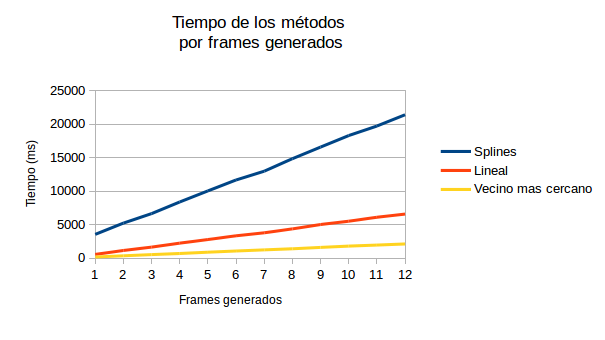
\includegraphics[scale= 0.6]{imagenes/aumentandoFramesToAdd.png}
  \end{center}
  \vspace{-10pt}
  \vspace{-10pt}
\end{wrapfigure}

Como vemos en el gráfico, el tiempo de procesamiento es lineal, esto es debido a que en cada iteración aumentamos la cantidad de frames a generar. Era de esperarse que un método como splines resultara ser el que más tarde en realizar su tarea, dado que realiza más operaciones que los otros métodos. \\

Por otro lado, realizamos una medición de tiempos con el mismo video, donde la cantidad de frames a generar es 1,   las dimensiones de los frames son fijas, y lo que variamos fue la cantidad de frames del video de entrada, aumentándolo de a 8 frames en cada medición. Para el video con movimiento, tomamos un segmento de un video largo tomando cada vez más frames, siempre desde el mismo frame original. Obtuvimos los siguientes resultados:


\begin{figure}[h!]
  \centering
    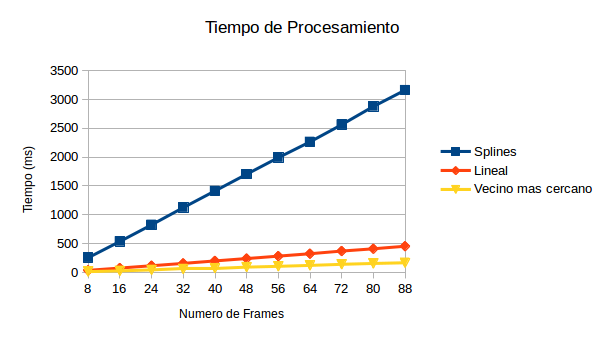
\includegraphics[scale= 0.8]{imagenes/aumentandoFramesMessi.png}
  \caption{Tiempo de Procesamiento agregando 1 frame aumentando la cantidad de frames originales}
\end{figure}

Los resultados que obtuvimos fueron lineales, como en el experimento anterior, con lo cual concluimos que la complejidad no depende únicamente de la cantidad de frames a generar, sino también de la cantidad de frames de entrada.\\


Intuitivamente el tiempo de procesamiento para cada método no debería variar si el video de prueba tiene gran movimiento o no, es decir, si hay mucha variacón del color de pixel entre frame y frame. Intuimos esto porque las operaciones que dependen del valor de un pixel son de tiempo constante (multiplicaciones, divisiones, sumas, restas y asignaciones). En particular, el video de prueba del experimento anterior, tenía una escena donde habia mucho movimiento, y esto no se reflejó en la medición temporal. \\

Por otro lado, tomamos los tiempo de procesamiento para un video del mismo ancho y largo que el video anterior, donde todos los frames eran blancos (todos los pixeles valen 255) tomando en cada medicion la misma cantidad de frames para poder ver efectivamente si los tiempos obtenidos eran menores, mayores o iguales. Los resultados obtenidos fueron muy parecidos al otro video, por lo que decidimos graficarlo tomando los tiempos del video con movimiento dividido el tiempo del video en blanco.

\begin{wrapfigure}{r}{0.6\textwidth}
  \vspace{-20pt}
  \begin{center}
    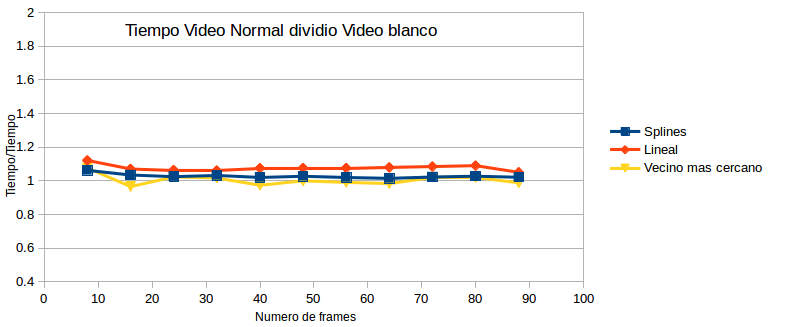
\includegraphics[scale= 0.6]{imagenes/aumentandoFramesMessiSobreWhite.png}
  \end{center}
  \vspace{-10pt}
  \vspace{-10pt}
\end{wrapfigure}

La mayor diferencia de tiempo entre ambos videos surgió en el método de splines. A pesar de no ser un tiempo significativamente distinto, creemos que la razón de que el tiempo sea ligeramente mayor en el video con movimiento radica en que los coeficientes de los polinomios obtenidos para el video en blanco son cero mientras que esto no sucede así para el otro video, haciendo que la evaluacion del polinomio sea más rápida.\\

Quedo por experimentar qué sucede con el tiempo cuando se varían ambos parámetros a la vez (frames generados y frames totales del video).



\subsection{Analisis de errores visuales por la aplicacion de los metodos}
\noindent Para esta sección utilizamos los siguiente videos:

$Gangnam Style:$ Video con cambios de cámara repentinos.

$Messi:$ Video con movimientos rápidos, sin cambios de cámara.

$Mario:$ Video del videojuego Super Mario Bros. Lo utilizamos por ser un video con movimientos rápidos, con el fin de poder observar diferencias visibles entre los métodos de 
interpolación.

$Tonalidad:$ Video de una suecesion de frames, donde cada frame es todo del mismo color, cambiando gradualmente de color, empezando desde el negro y terminando en el blanco. Lo utilizamos para ver las diferencias de colores generadas entre el método lineal y splines.\\

Primero utilizamos el video de $Gangnam Style$ para analizar los artifacts producidos por los cambios bruscos de cámara. El video tiene 3 cambios de cámara en 4 segundos. Ejecutamos los 3 métodos agregando 1 frame de por medio y comparamos las imágenes generadas justo en los cambios de cámara. Uno de ellos es el que se ve en la imágen. 

\newpage

%gangman:
\begin{figure}[h!]
  \centering
    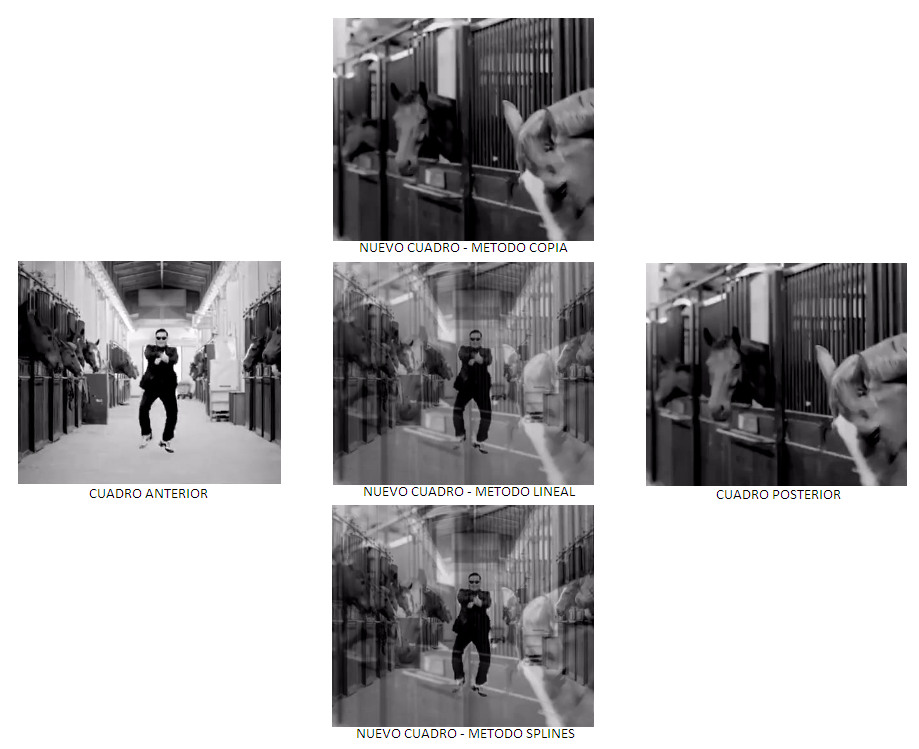
\includegraphics[scale= 0.5]{imagenes/gangman.png}
  \caption{Errores visuales por cambio de cámara}
\end{figure}


Como se puede ver en la Figura, el cambio brusco de camara genera frames intermedios no satisfactorios, donde parecería haber varios frames superpuestos y ligeramente corridos, mientras que con vecino más cercano no se ve este artifact, aunque obviamente se pierde cierta fluidez en el video en su totalidad.
Una posible manera de subsanar este artifact sería calculando la diferencia entre 2 frames, y si es más alta que cierto threshold, se considera que hubo un cambio brusco de camara, y en vez de calcular el polinomio interpolador entre esos 2 frames, se utiliza vecino más cercano.\\

Ahora queremos ver qué pasa cuando hay movimientos rápidos en alguna parte o en la totalidad del video, sin movimientos de cámara. Para esto utilizamos los videos de $Messi$ y de $Mario$. Para el video de $Messi$ interpolamos un único frame de por medio, y para el video de $Mario$, 5 frames. 

\newpage

\begin{figure}[h!]
  \centering
    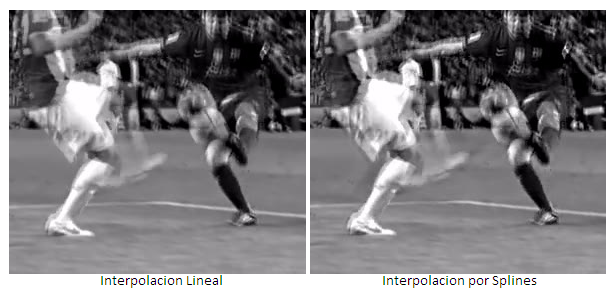
\includegraphics[scale= 0.5]{imagenes/messi.png}
  \caption{Errores visuales por rápidos movimientos}
\end{figure}


%messi:
No se pudieron apreciar diferencias significativas entre interpolacion lineal y splines. Ambos otorgan el mismo grado de fluidez al video. En el caso del vecino más cercano, cuando hay mucho movimiento, el video se ve muy cortado. Esto no se puede ver en las imágenes, pero en el video la diferencia es muy notoria.


\begin{figure}[h!]
  \centering
    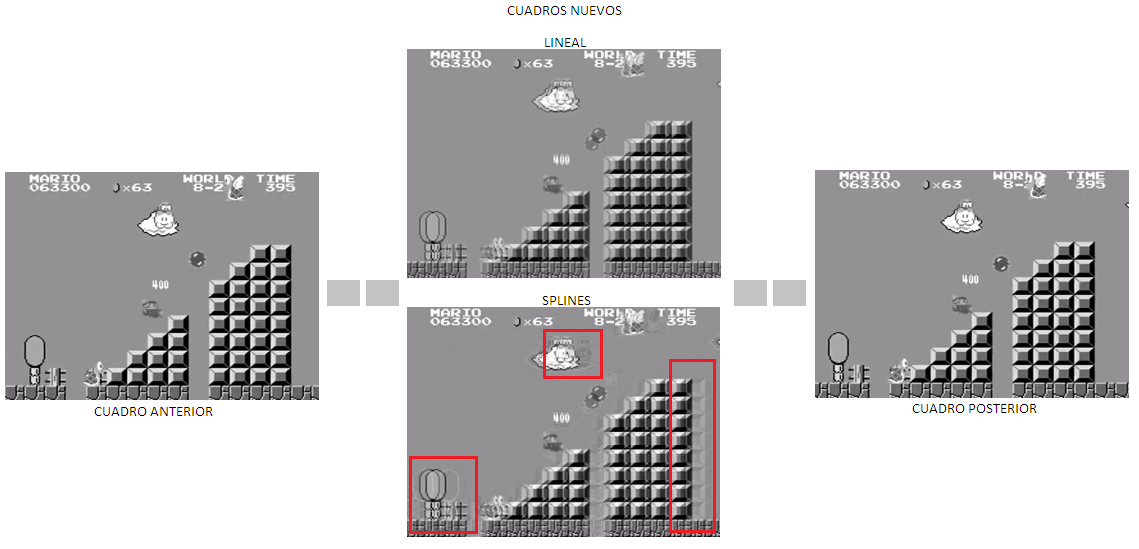
\includegraphics[scale= 0.587]{imagenes/mario.png}
  \caption{Errores visuales por rápidos movimientos}
\end{figure}


%mario:
En el video del $Mario$ al aplicar los metodos de interpolación, observamos diferencias claras entre ambos métodos. En la interpolación con splines, se puede ver que en los frames generados queda una suerte de blur que no está presente en los frames generados por interpolación lineal (zonas marcadas en rojo), lo que nos da a entender que en la interpolación por splines se esta utilizando mas información de los frames anteriores para generar el nuevo frame, otorgando visualmente una mayor fluidez al video.
Este efecto es más notorio mientras más frames se generan mediante interpolación. En el mismo video con 1 frame generado de por medio no se puede apreciar tanto esta diferencia.\\

También realizamos otro experimento con el video $Tonalidad$ (para el cual no agregamos imagenes ya que a simple vista no eran muy informativas de lo que estaba pasando) que consistió en un video generado por nosotros, el cual iba pasando por distintas tonalidades, empezando por el negro y aclarandose más hasta llegar al blanco. En este caso interpolación lineal y splines dieron diferentes, aunque fue una diferencia tan sutil que solo pudimos observarla comparando los valores de los píxeles con GIMP.\\

Tanto interpolación lineal como interpolación por splines dan resultados visualmente similares, salvo en el caso en que se generen muchos frames con interpolación.

\newpage
\subsection{Experimentación PSNR}

En esta sección analizamos las mediciones con el error cuadrático medio (ECM) y el Peak Signal to Noise Ratio (PSNR) y analizamos el impacto de los aspectos cualitativos de los vídeos en los métodos propuestos. \\

En el siguiente experimento, tomamos un video y le quitamos frames de a 1, para luego generarlos. Estudiamos como varía dicho índice comparando los frames originales que quitamos y los frames generados que los reemplazan. Utilizamos un video con cambios de cámara repentinos para poder ver como se comportan los métodos y ver el PSNR obtenido en esos cortes. Para esto, utilizamos un segmento del video $Gangnam Style$ que posee estas cualidades.
Los resultados que obtuvimos fueron los siguientes:


\begin{figure}[h!]
  \caption{Gráfico del PSNR comparando contra frames originales}
  \centering
    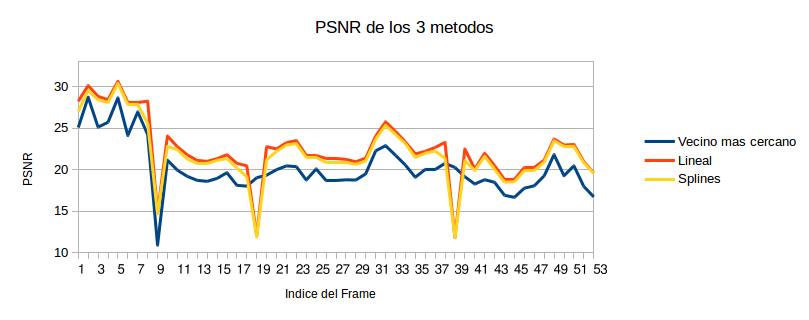
\includegraphics[scale=0.5]{imagenes/PSNRGangnam.png}
\end{figure}

Los picos inferiores del gráfico se corresponden con los frames donde ocurre un cambio de toma brusco. El pico más bajo corresponde al método del vecino más cercano, como esperabamos. Sin embargo, no sucede lo mismo con los otros dos picos. Esto se debe a que para esos frames, el algoritmo seleccinó los frames posteriores al cambio de toma, teniendo así una menor diferencia que los otros métodos.\\

Es interesante tambien ver qué sucede con los errores cuando agregamos muchos frames nuevos generados con los métodos. Usamos para este experimento un video con poco movimiento en los frames pero con movimientos rápidos ($Mario$). Aplicamos cada uno de los métodos generando 8 frames por cada 2 originales, y comparamos los frames generados con los frames que se quitaron, utilizando la medida de PSNR.

\begin{figure}[h!]
  \caption{Gráfico del PSNR comparando contra frames originales}
  \centering
    \includegraphics[scale=0.5]{imagenes/PSNR3metodosmario.png}
\end{figure}


Los picos que se ven en las tres funciones corresponden con frames nuevos que estaban más cerca de los frames originales es decir, se tiene mayor error al generar los frames que estan más alejados. Se corresponden tambien con los puntos de inflexión de los polinomios cúbicos que se usan para aproximarlos.\\

Tambien vemos que para este video en particular y cuando se generan muchos frames nuevos, el método de interpolación lineal funciona mejor si se mira cada imagen por separado. Sin embargo, cuando vemos el video generado por el método de splines los movimientos parecen ser mas fluidos y realistas. La medida de PSNR es más bien utilizada para medir la calidad de una imagen reconstruida por compresión y descompresión o para medir la calidad de una señal. Es por eso que no puede medir como queremos la calidad del movimiento.\\


Ahora vamos a analizar cual es la diferencia del error producido al agregar más o menos frames intermedios. En el experimento anterior agregamos una cantidad fija de frames y vimos como se comportaba el PSNR, ahora vamos a analizar la diferencia del error agregando 1 o 5 frames intermedios. Para esto, calculamos el PSNR del tercer frame de los 5 generados, y de los frames generados de a 1 que correspondían con los anteriores. 

\begin{figure}[h!]
  \caption{Gráfico del PSNR comparando contra frames originales con diferentes cantidades de frames agregados}
  \centering
    \includegraphics[scale=0.5401]{imagenes/PSNR1y5framesagregados.png}
\end{figure}

Como ya habíamos notado antes, la introducción de más frames entre cada par de frames originales aumenta el $"$ruido$"$ de la señal (que en este caso se puede interpretar como una imagen), lo cual se ve reflejado en una disminución en el PSNR, ya que aumenta el ECM debido al ruido. Sin embargo, no pudimos determinar la razón de los bajos valores de PSNR en los primeros frames generados.\\

Lo que quedo por experimentar es qué sucede cuando se realiza interpolación por splines variando el tamaño fijo de los bloques, y qué sucede cuando los tamaños del bloque son variables para una misma instancia.

%grafico de medicion de ecm con 
% \begin{wrapfigure}{r}{0.6\textwidth}
%   \vspace{-20pt}
%   \begin{center}
%     \includegraphics[scale= 0.6]{imagenes/.png}
%   \end{center}
%   \vspace{-10pt}
%   \vspace{-10pt}
% \end{wrapfigure}







\newpage

\section{Conclusiones}

En este trabajo pudimos ver una aplicación real para los métodos de interpolación más comunes, lineal y cúbico. Analizamos el comportamiento de cada método para una serie de videos específicos, y pudimos comprobar que, aunque el PSNR da menor en el método de splines, esto no significa necesariamente que el video pierda fluidez, lo que si pasa en el método del vecino más cercano.\\

A pesar de que nosotros vimos los errores (artifacts) que se produjeron en cuadros específicos, esto no es tan notorio en el video que se genera, aunque si se agregan demasiados frames, el video comienza a verse borroso y molesto a la vista. También vimos que en algunos casos los artifacts se pueden arreglar haciendo alguna pequeña modificación en el algoritmo, como en el caso de los artifacts producidos por los cambios de cámara.\\

Un aspecto que nos pareció interesante, fue el hecho de que el uso de estos algoritmos para la generación de videos en cámara lenta, puede ahorrar dinero en la compra de cámaras que posean dicha funcionalidad incorporada, y puede también ahorrar tiempo de transferencia entre la cámara y el centro de cómputos. Además, vimos que la complejidad temporal es lineal con respecto a la cantidad de frames.
\newpage

\section{Apéndice A: Enunciado}

%\usepackage[ruled,vlined]{algorithm2e}

%\parindent = 0 pt
\parskip = 5 pt

\newcounter{row}
\newcounter{col}

\newcommand\setrow[3]{
	\setcounter{col}{1}
	\foreach \n in {#1, #2, #3} {
	\edef\x{\value{col} - 0.5}
	\edef\y{3.5 - \value{row}}
	\node[anchor=center] at (\x, \y) {\n};
	\stepcounter{col}
	}
	\stepcounter{row}
}

\newcommand\setrowaux[7]{
	\setcounter{col}{1}
	\foreach \n in {#1, #2, #3, #4, #5, #6, #7} {
	\edef\x{\value{col} - 0.5}
	\edef\y{7.5 - \value{row}}
	\node[anchor=center] at (\x, \y) {\n};
	\stepcounter{col}
	}
	\stepcounter{row}
}

\newcommand{\real}{\mathbb{R}}

%\begin{document}
\begin{center}
\begin{tabular}{r|cr}
 \begin{tabular}{c}
{\large\bf\textsf{\ M\'etodos Num\'ericos\ }}\\ 
Segundo Cuatrimestre 2015\\
{\bf Trabajo Pr\'actico 3}\\
\end{tabular} &
\begin{tabular}{@{} p{1.6cm} @{}}

\includegraphics[width=1.6cm]{logodpt.jpg}
\end{tabular} &
\begin{tabular}{l @{}}
 \emph{Departamento de Computaci\'on} \\
 \emph{Facultad de Ciencias Exactas y Naturales} \\
 \emph{Universidad de Buenos Aires} \\
\end{tabular} 
\end{tabular}
\vskip 10pt
\textbf{\Large \emph{Un juego de niños}}\\
\vspace{0.5cm}
\end{center}

\vskip 10pt
\hrule
\vskip 5pt

{\bf\noindent Introducci\'on}

¿Quién nunca ha visto un video gracioso de bebés? El éxito de esas producciones audiovisuales ha sido tal que el sitio youborn.com es uno de los más visitados diariamente. Los dueños de este gran sitio, encargado de la importantísima tarea de llevar videos graciosos con bebés a todo el mundo, nos ha pedido que mejoremos su sistema de reproducción de videos.

Su objetivo es tener videos en cámara lenta (ya que todos deseamos tener lujo de detalle en las expresiones de los chiquilines en esos videos) pero teniendo en cuenta que las conexiones a internet no necesariamente son capaces de transportar la gran cantidad de datos que implica un video en \textit{slow motion}. La gran idea es minimizar la dependencia de la velocidad de conexi\'on y s\'olo enviar el video original. Una vez que el usuario recibe esos datos, todo el trabajo de la cámara lenta puede hacerse de modo offline del lado del cliente, optimizando los tiempos de transferencia. Para tal fin utilizaremos técnicas de interpolación, buscando generar, entre cada par de cuadros del video original, otros ficticios que nos ayuden a generar un efecto de slow motion.


\vskip 5pt

{\bf\noindent Definici\'on del problema y metodolog\'ia}

Para resolver el problema planteado en la secci\'on anterior, se considera el siguiente contexto. Un video está compuesto por cuadros (denominados también \textit{frames} en inglés) donde cada uno de ellos es una imagen. Al reproducirse rápidamente una después de la otra percibimos el efecto de movimiento a partir de tener un ``buen frame rate'', es decir una alta cantidad de cuadros por segundo o fps (frames per second). Por lo general las tomas de cámara lenta se generan con cámaras que permiten tomar altísimos números de cuadros por segundo, unos 100 o m\'as en comparaci\'on con entre 24 y 30 que se utilizan normalmente. 

En el caso del trabajo práctico crearemos una cámara lenta sobre un video grabado normalmente. Para ello colocaremos más cuadros entre cada par de cuadros consecutivos del video original de forma que representen la información que debería haber en la transición y reproduciremos el resultado a la misma velocidad que el original. Las im\'agenes correspondientes a cada cuadro est\'an conformadas por p\'ixeles. En particular, en este trabajo utilizaremos im\'agenes en escala de grises para disminuir los costos en tiempo necesarios para procesar los datos y simplificar la implementaci\'on; sin embargo, la misma idea puede ser utilizada para videos en color. 

El objetivo del trabajo es generar, para cada posici\'on $(i,j)$, los valores de los cuadros agregados en funci\'on de los cuadros conocidos. Lo que haremos ser\'a interpolar en el tiempo y para ello, se propone considerar al menos los siguientes tres m\'etodos de interpolaci\'on:

\begin{enumerate}
\item \emph{Vecino m\'as cercano:} Consiste en rellenar el nuevo cuadro replicando los valores de los p\'ixeles del cuadro original que se encuentra más cerca. \label{item:nn}
\item \emph{Interpolaci\'on lineal:} Consiste en rellenar los p\'ixeles utilizando interpolaciones lineales entre p\'ixeles de cuadros originales consecutivos. \label{item:lineal}
\item \emph{Interpolaci\'on por Splines:} Simliar al anterior, pero considerando interpolar utilizando splines y tomando una cantidad de cuadros mayor. Una alternativa a considerar es tomar la informaci\'on de bloques de un tama\~no fijo (por ejemplo, 4 cuadros, 8 cuadros, etc.), con el tama\~no de bloque a ser determinado experimentalmente. \label{item:spline}
\end{enumerate}


Cada m\'etodo tiene sus propias caracter\'isticas, ventajas y desventajas particulares. Para realizar un an\'alisis cuantitativo, llamamos $F$ al frame del video real (ideal) que deber\'iamos obtener con nuestro algoritmo, y sea $\bar{F}$ al frame del video efectivamente construido. Consideramos entonces dos medidas, directamente relacionadas entre ellas, como el \emph{Error Cuadr\'atico Medio} (ECM) y \emph{Peak to Signal Noise Ratio} (PSNR), denotados por $\texttt{ECM}(F,\bar{F})$ y $\texttt{PSNR}(F,\bar{F})$, respectivamente, y definidos como:
\begin{equation}
\texttt{ECM}(F,\bar{F}) = \frac{1}{mn}\sum_{i=1}^m\sum_{j = 1}^n |F_{k_{ij}} - \bar{F}_{k_{ij}}|^2 \label{eq:ecm}
\end{equation}
\noindent y
\begin{equation}
\texttt{PSNR}(F,\bar{F}) = 10 \log_{10}\bigg(\frac{255^2}{\texttt{ECM}(F,\bar{F})}\bigg). \label{eq:psnr}
\end{equation}

Donde $m$ es la cantidad de filas de p\'ixeles en cada imagen y $n$ es la cantidad de columnas. Esta métrica puede extenderse para todo el video.

En conjunto con los valores obtenidos para estas m\'etricas, es importante además realizar un an\'alisis del tiempo de ejecuci\'on de cada m\'etodo y los denominados \emph{artifacts} que produce cada uno de ellos. Se denominan \emph{artifacts} a aquellos errores visuales resultantes de la aplicaci\'on de un m\'etodo o t\'ecnica. La b\'usqueda de este tipo de errores complementa el estudio cuantitativo mencionado anteriormente incorporando un an\'alisis cualitativo (y eventualmente subjetivo) sobre las im\'agenes generadas.

\vskip 5pt

{\bf\noindent Enunciado}

Se pide implementar un programa en \verb-C- o \verb-C++- que implemente como m\'inimo los tres m\'etodos mencionados anteriormente y que dado un video y una cantidad de cuadros a agregar aplique estas t\'ecnicas para generar un video de cámara lenta. A su vez, es necesario explicar en detalle c\'omo se utilizan y aplican los m\'etodos descriptos en \ref{item:nn}, \ref{item:lineal} y \ref{item:spline} (y todos aquellos otros m\'etodos que decidan considerar opcionalmente) en el contexto propuesto. Los grupos deben a su vez plantear, describir y realizar de forma adecuada los experimentos que consideren pertinentes para la evaluaci\'on de los m\'etodos, justificando debidamente las decisiones tomadas y analizando en detalle los resultados obtenidos as\'i como tambi\'en plantear qu\'e pruebas realizaron para convencerse de que los m\'etodos funcionan correctamente.


{\bf\noindent Programa y formato de entrada}

Se deberán entregar los archivos fuentes que contengan la resolución del trabajo práctico. El ejecutable tomará cuatro parámetros por línea de comando que serán el archivo de entrada, el archivo de salida, el método a ejecutar (0 para vecinos más cercanos, 1 para lineal, 2 para splines y otros números si consideran más métodos) y la cantidad de cuadros a agregar entre cada par del video original.

Tanto el archivo de entrada como el de salida tendrán la siguiente estructura:

\begin{itemize}
  \item En la primera línea está la cantidad de cuadros que tiene el video (\verb|c|).
  \item En la segunda línea está el tamaño del cuadro donde el primer número es la cantidad de filas y el segundo es la cantidad de columnas (\verb|height width|).
  \item En la tercera línea está el framerate del video (\verb|f|).
  \item A partir de allí siguen las imágenes del video una después de la otra en forma de matriz. Las primeras \verb|height| l\'ineas son las filas de la primera imagen donde cada una tiene \verb|width| n\'umeros correspondientes a los valores de cada píxel en esa fila. Luego siguen las filas de la siguiente imagen y as\'i sucesivamente.
\end{itemize}

Además se presentan herramientas en Matlab para transformar videos (la herramienta fue probada con la extensión .avi pero es posible que funcione para otras) en archivos de entrada para el enunciado y archivos de salida en videos para poder observar el resultado visualmente. También se recomienda leer el archivo de README sobre la utilización.


\vskip 0.5 cm
\hrule
\vskip 0.2 cm

{\bf Sobre la entrega}
\begin{itemize}
\item \textsc{Formato electr\'onico:} Martes 10 de Noviembre de 2015, {\bf{\underline{hasta las 23:59}}}, enviando el trabajo
(\texttt{informe} + \texttt{c\'odigo}) a \texttt{metnum.lab@gmail.com}. El \texttt{asunto} del email debe comenzar con el texto \verb|[TP3]| seguido
de la lista de apellidos de los integrantes del grupo. Ejemplo: \texttt{[TP3] Artuso, Belloli, Landini}
\item \textsc{Formato f\'isico:} Mi\'ercoles 11 de Noviembre de 2015, en la clase pr\'actica.
\end{itemize}


%\end{document}

\section{Referencias}

\begin{itemize}
\item $[$BUR9$]$ Numerical Analysis 9th Edition - Burden, Faires.
\end{itemize}
%\newpage



\bibliographystyle{plain}
\bibliography{tp3}

\end{document}
